\documentclass{article}

\usepackage{header}
\newcommand{\equivclass}[1]{%
  #1/{\sim}%
}

\usepackage[left=2cm,right=2cm, top=2cm,bottom=2cm,bindingoffset=0cm]{geometry}

\usepackage{graphicx}
\graphicspath{.}

\usepackage{hyperref}  % so the reference URLs and citations are clickable
\usepackage{csquotes}  % needed for biblatex for babel
\usepackage[backend=biber]{biblatex}
\addbibresource{bibliography.bib}

\usepackage{titlepage}

\setUDK{004.9}
\setToResearch

\setTitle{Магнитуда некоторых гибридных многообразий}

% Выбрать одно из трех:
% КТ1 -- \setStageOne
% КТ2 -- \setStageTwo
% Финальная версия -- \setStageFinal
%\setStageOne
%\setStageTwo
\setStageFinal

\setGroup{204}
%сюда можно воткнуть картинку подписи
% \setStudentSgn{\smash{\includegraphics[scale=0.25]{my-sig.png}}}
% \setStudentSgn{\includegraphics[scale=0.10]{my-sig.jpg}}
% \setStudentSgn{\smash{kjdfl}}
\setStudent{М.М.Марченко}
\setStudentDate{29.08.2023}
\setAdvisor{Всеволод Леонидович Чернышев}
\setAdvisorTitle{Доцент} %(научно-учебная лаборатория методов анализа больших данных)}
\setAdvisorAffiliation{НИУ ВШЭ, ФКН, Департамент больших данных и информационного поиска}
\setAdvisorDate{}
\setGrade{}
%сюда можно воткнуть картинку подписи
\setAdvisorSgn{}
\setYear{2023}

\begin{document}

% Эта команда создает титульную страницу
\makeTitlePage

% Здесь будет автоматически генерироваться содержание документа
\tableofcontents

% Данное окружение оформляет аннотацию: краткое описание текста выделенным абзацем после заголовка
%\begin{abstract}
%    Проект в реализации теории,
%\end{abstract}
\section{Project description}

As a continuation of my previous coursework which approximated magnitude function
of a metric graph, as a summer project I decided to keep on working within the same theme by 
attempting to finish the calculations of magnitude of three types of hybrid manifolds
from another students thesis.
\\

Despite not obtaining any magnitude values as a result of calculations, this summer
project had been a productive and valuable practice for me --- for the first time
I came across Riemannian manifolds and hybrid manifolds, tried using Laplace's
method to evaluate magnitude function asymptotics, got familiar with another approach
for finding magnitude and revised a few mathematical analysis and optimization methods topics. 
\\

This report leaves out the calculations attempts (since they are unsuccessful) and
focuses on definitions and approaches which were new to me.

\section{Preliminaries}
\subsection{Magnitude}

The definition which I used for my coursework for approximating magnitude by computer simulations is given below (as it appears in \textcite{calc}):

\begin{definition}
\item
    $\text{Let $X$ be a finite metric space with metric $d$. If $\forall x \in X \  \exists \  w_x$(also called weightening) : }$ 
    $$\forall x \in X : \sum_{x' \in X} w_{x'} \cdot e^{-d(x, x')} = 1$$
    $\text{then magnitude of $X$ is }$
    $$\mathcal{M}(X) \coloneqq \sum_{x \in X} w_x $$ 
\item
\end{definition}
\begin{remark}
\item
    $\text{If $Z$ is a $|X| \cross |X|$ matrix, with values $Z_{i, j} = e^{-d(x_i, x_j)}$, where $x_i, x_j \in X$ and Z is invertible, then:}$
\item
    $$\mathcal{M}(X) = \sum_{i, j} (Z^{-1})_{i, j} $$
\end{remark}

The following definition, which I found out only during this project, is useful for
more analytical (rather than computational) approach and was shown in \textcite{Meckes_2012}. 

\begin{definition}
\item 
Let $X$ be a finite metric space with metric $d$ and a measure $\nu$ defined on $X$, such that:
    $$\forall y \in X : \int_{x \in X} e^{-d(x, y)} d \nu(x) = 1$$
then magnitude of $X$ is 
    $$\mathcal{M}(X) = \nu(X)$$
\item 
\end{definition}

\subsubsection{Possible algorithm for finding magnitude}

As 2nd definition of magnitude states, we need to find a measure satisfying the
condition given above. Since linear combination of measures is still a measure we
can try to find suitable measure by undetermined coefficients method, using known
ones: 
Lebesgue measures (length for intervals, area for hybrid manifolds) and Dirac
measures (usually used for indication of gluing points). 
\\

After calculating integrals for different cases of $y \in X$ (as in 2nd definition),
we can attempt finding coefficients from obtained equations and in case of success 
calculate the resulting measure of $X$. 
\\

For example for metric tree the resulting measure will be equal to
$$\nu = \frac{1}{2} \sum_{e \in E(X)} \mu_{e} + \sum_{v \in V(X)} (1 - \frac{1}{2} \text{deg}(v)) \delta_{v}$$ 
($\mu_e$ is Lebesgue for each edge and $\delta_x$ is Dirac for each vertex)
\\
meaning that magnitude equals to 
$$\mathcal{M}(X) = \nu(X) = \frac{\sum w_e}{2} + 1$$

\subsubsection{Magnitude function}
\begin{definition}
    $\text{If } X \text{ is a metric space with metric $d(x, y)$ and $t \in (0, \infty)$ then } tX \text{ is a metric space with metric } t \cdot d(x, y)$
\end{definition}
\begin{definition}
    $f_{\mathcal{M}} : (0, \infty) \rightarrow \mathbb{R} \text{ is a magnitude function of X, if }$
    $$f_{\mathcal{M}}(t) = \mathcal{M}(tX)$$
\end{definition}

\textbf{Illustration of magnitude function for a three point space with the following distances:}
\\ Note how the values of the magnitude function correspond to the number of points seen if we change the perspective: first we see 1 point, then 2 as we get closer but still see two of them as one, then 3.
\begin{center}
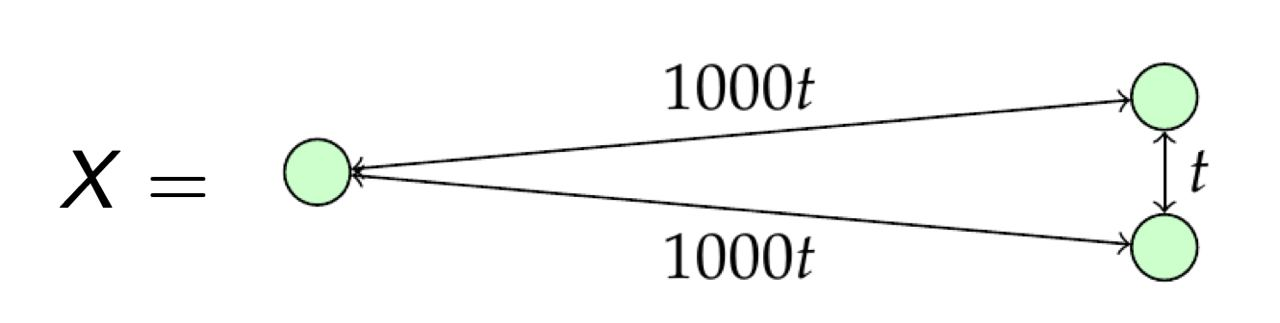
\includegraphics[width=.4\textwidth]{3dots} \\ 
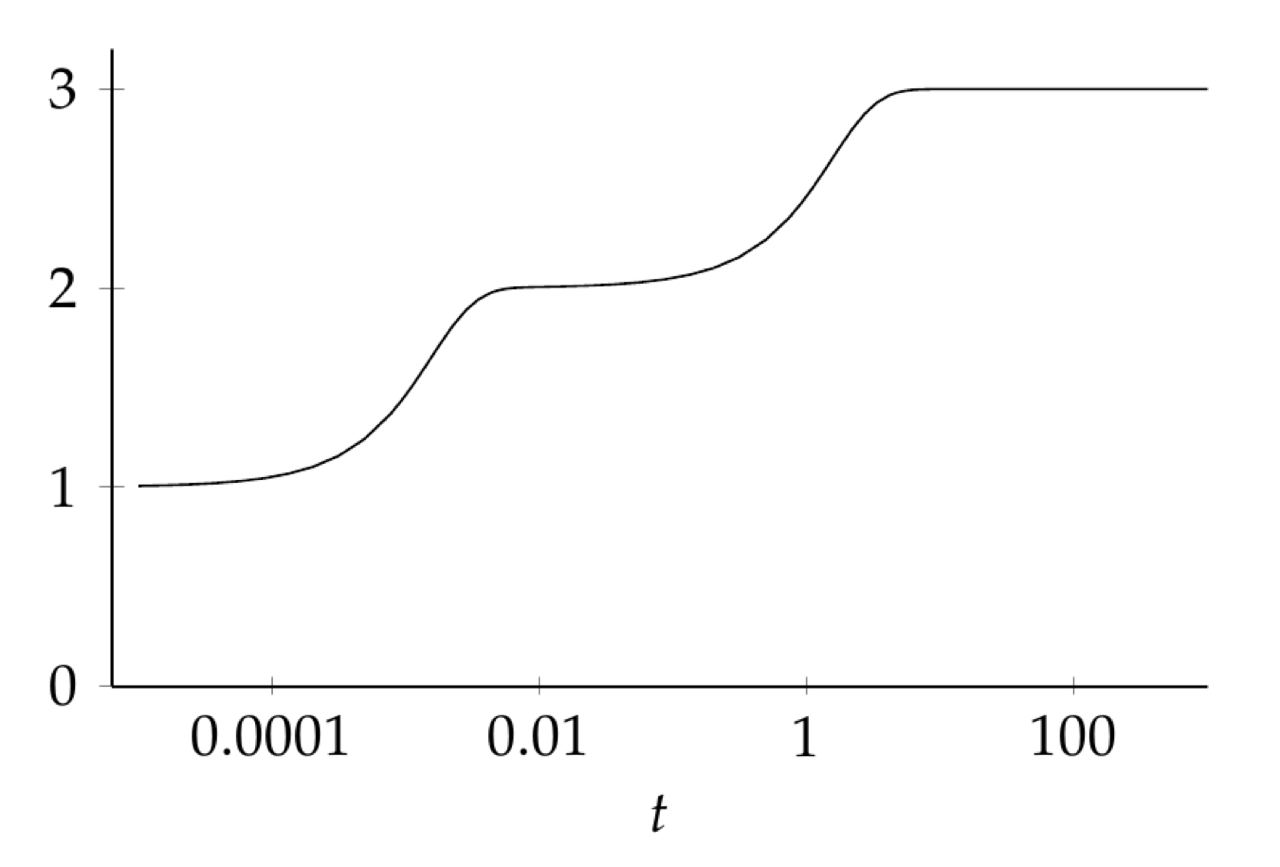
\includegraphics[width=.35\textwidth]{mfunc3dots}
\end{center}

\subsection{Hybrid manifolds}

    
\begin{definition} (coming from \textcite{Pankrashkin_2011})
Let $M_1, M_2, ..., M_k$ be a set of compact Riemannian manifolds, and $L_1, L_2, ..., L_n$ a set of segments. 
    On manifolds we choose $2n$ points, each of them we glue (construct a bijection)
    to one of the segments at one of its ends. The resulting metric space with shortest path metric is a hybrid manifold. 
\end{definition}

Note, that metric graph is a simplest hybrid manifold with each $M_i$ being a point. 
In thesis, that this project was based on, author studies 3 simple hybrid manifolds, 
each with case $n = k = 1$, and $M_1$ being sphere, cylinder and torus respectively. 
\\

For each of the cases author reviews the value of $d(x, y)$ to find the undetermined
coefficients of the measure expression, but due to big number of cases and complicated 
integrals the calculations are hard to compute.
\subsection{Laplace's method}

As mentioned earlier to calculate magnitude we need to calculate (or at least approximate)
integrals of the form
$$\int_{x \in X} e^{t \cdot (-d(x, y))} dx$$
We added $t$ since the idea was to calculate magnitude function (particularly its
asymptotics) rather than magnitude. Besides $x$ can be multidimensional, as in
case of all three examined manifolds it is 2-dimensional.
\\

To approximate this integral we can use multivariate case of Laplace's method (from \textcite{fedor}):
$$\text{If } x = (x_1, ..., x_d); \ f: \mathbb{R}^d \rightarrow \mathbb{R} \text{ and } x_0 \in X : f(x_0) \text{ - maximum on X, then}$$
$$\int_{x \in X} e^{M \cdot f(x)} dx \approx \left( \frac{2\pi}{M} \right)^{\frac{d}{2}} \frac{e^{M \cdot f(x_0)}}{|-H(f)(x_0)|^{\frac{1}{2}}} = g(M) \text{ as } M \rightarrow \infty $$
where $|H|$ is Hessian determinant.
\\

$\approx $ in this case means that $\lim_{M\to\infty} \frac{\int_{x \in X} e^{M \cdot f(x)}}{g(M)} = 1$ so we can evaluate asymptotics of magnitude as a result. 

\section{Conclusions and future work}
As already mentioned above I did not obtain any results due to short duration of 
summer projects, but I do plan to continue this project in the future. 
\\

My plan is the following: using Laplace's method from the last section on different cases of integrals presented
in the thesis this project is based on, for every scaling factor I hope to obtain 
a system of equations which solutions will approximate the undetermined coefficients
as scaling factor goes to infinity. Thus, substituting these solutions into the measure
integral which on infinity would be asymptotically equivalent to the magnitude function.
\\

All in all, the project was interesting and challenging to me as it is the first time I was 
given a task of figuring out and continuing someone else's work, besides it dealt with a combination of
new topics.
\printbibliography

% Проведем небольшой обзор возможностей \LaTeX. Далее идет обзорный кусок, который надо будет вырезать. Он приведен лишь для демонстрации возможностей \LaTeX.
%
% \section{Нумеруемый заголовок}
% Текст раздела
% \subsection{Нумеруемый подзаголовок}
% Текст подраздела
% \subsubsection{Нумеруемый подподзаголовок}
% Текст подподраздела
%
% \section*{Не нумеруемый заголовок}
% Текст раздела
% \subsection*{Не нумеруемый подзаголовок}
% Текст подраздела
% \subsubsection*{Не нумеруемый подподзаголовок}
% Текст подподраздела
%
%
% \paragraph{Заголовок абзаца} Текст абзаца
% Формулы в тексте набирают так $x = e^{\pi i}\sqrt{\text{формула}}$. Выключенные не нумерованные формулы набираются либо так:
% \[
% x = e^{\pi i}\sqrt{\text{формула}}
% \]
% Либо так
% $$
% x = e^{\pi i}\sqrt{\text{формула}}
% $$
% Первый способ предпочтительнее при подаче статей в журналы AMS, потому рекомендую привыкать к нему.
%
% Выключенные нумерованные формулы:
% \begin{equation}
% \label{Equation1}
% % \label{имя-метки} эта команда ставит метку, на которую потом можно сослаться с помощью \ref{имя-метки}. Метки можно ставить на все объекты, у которых есть автоматические счетчики (номера разделов, подразделов, теорем, лемм, формул и т.д.
% x = e^{\pi i}\sqrt{\text{формула}}
% \end{equation}
% Или не нумерованная версия
% \begin{equation*}
% x = e^{\pi i}\sqrt{\text{формула}}
% \end{equation*}
%
% Уравнение \ref{Equation1} радостно занумеровано.
%
% Лесенка для длинных формул
% \begin{multline}
% x = e^{\pi i}\sqrt{\text{очень очень очень длинная формула}}=\\
% \tr A - \sin(\text{еще одна очень очень длинная формула})=\\
% \cos z \Im \varphi(\text{и последняя длинная при длинная формула})
% \end{multline}
%
% Многострочная формула с центровкой
% \begin{gather}
% x = e^{\pi i}\sqrt{\text{очень очень очень длинная формула}}=\\
% \tr A - \sin(\text{еще одна очень очень длинная формула})=\\
% \cos z \Im \varphi(\text{и последняя длинная при длинная формула})
% \end{gather}
%
% Многострочная формула с ручным выравниванием. Выравнивание идет по знаку $\&$, который на печать не выводится.
% \begin{align}
% x = &e^{\pi i}\sqrt{\text{очень очень очень длинная формула}}=\\
% &\tr A - \sin(\text{еще одна очень очень длинная формула})=\\
% &\cos z \Im \varphi(\text{и последняя длинная при длинная формула})
% \end{align}
%
% \begin{theorem}
% Текст теоремы
% \end{theorem}
% \begin{proof}
% В специальном окружении оформляется доказательство.
% \end{proof}
%
% \begin{theorem}[Имя теоремы]
% Текст теоремы
% \end{theorem}
% \begin{proof}[Доказательство нашей теоремы]
% В специальном окружении оформляется доказательство.
% \end{proof}
%
% \begin{definition}
% Текст определения
% \end{definition}
%
% \begin{remark}
% Текст замечания
% \end{remark}
%
% \paragraph{Перечни:} Нумерованные
% \begin{enumerate}
% \item Первый
% \item Второй
% \begin{enumerate}
% \item Вложенный первый
% \item Вложенный второй
% \end{enumerate}
% \end{enumerate}
%
% Не нумерованные
%
% \begin{itemize}
% \item Первый
% \item Второй
% \begin{itemize}
% \item Вложенный первый
% \item Вложенный второй
% \end{itemize}
% \end{itemize}
\end{document}
